\documentclass[11pt,oneside,letterpaper]{article}

% graphicx package, useful for including eps and pdf graphics
\usepackage{graphicx}
\DeclareGraphicsExtensions{.pdf,.png,.jpg}

% basic packages
\usepackage{color}
\usepackage{parskip}
\usepackage{float}

% text layout
\usepackage{geometry}
\geometry{textwidth=15cm} % 15.25cm for single-space, 16.25cm for double-space
\geometry{textheight=22cm} % 22cm for single-space, 22.5cm for double-space

% helps to keep figures from being orphaned on a page by themselves
\renewcommand{\topfraction}{0.85}
\renewcommand{\textfraction}{0.1}

% bold the 'Figure #' in the caption and separate it with a period
% Captions will be left justified
\usepackage[labelfont=bf,labelsep=period,font=small]{caption}

% review layout with double-spacing
%\usepackage{setspace}
%\doublespacing
%\captionsetup{labelfont=bf,labelsep=period,font=doublespacing}

% cite package, to clean up citations in the main text. Do not remove.
\usepackage{cite}
%\renewcommand\citeleft{(}
%\renewcommand\citeright{)}
%\renewcommand\citeform[1]{\textsl{#1}}

% Remove brackets from numbering in list of References
\renewcommand\refname{\large References}
\makeatletter
\renewcommand{\@biblabel}[1]{\quad#1.}
\makeatother

\usepackage{authblk}
\renewcommand\Authands{ \& }
\renewcommand\Authfont{\normalsize \bf}
\renewcommand\Affilfont{\small \normalfont}
\makeatletter
\renewcommand\AB@affilsepx{, \protect\Affilfont}
\makeatother

% notation
\usepackage{amsmath}
\usepackage{amssymb}

%%% TITLE %%%
\title{\vspace{1.0cm} \Large \bf
ncov-forecasting-fit (title TBD)
}

\author[1,2]{Eslam Abousamra*}
\author[1,3]{Marlin Figgins*}
\author[1,2,4]{Trevor Bedford}

\affil[1]{Vaccine and Infectious Disease Division, Fred Hutchinson Cancer Center, Seattle, WA, USA}
\affil[2]{Department of Epidemiology, University of Washington, Seattle, WA, USA}
\affil[3]{Department of Applied Mathematics, University of Washington, Seattle, WA, USA}
\affil[4]{Howard Hughes Medical Institute, Seattle, WA, USA}


\date{}

\begin{document}

\maketitle

%%% ABSTRACT %%%
\begin{abstract}

Todo

\end{abstract}

%%% INTRODUCTION %%%
\section*{Introduction}

Modeling infectious diseases plays a key role in predicting growth of epidemics.
Understanding the trends and characteristics of emerging epidemics can guide public health officials to control their spread [Ding et al., 2021].
Epidemiologists face a multitude of challenges in order to provide accurate and timely predictions of disease spread.
With the increased availability of genomic sequencing, there has been efforts and potential in using sequences as a tool for investigating the genetic diversity, evolution, and transmission of epidemic-causing pathogens [Gire SK et al., 2014, Zhou et al., 2020]. 
More recently, with the deluge of data from various sources, issues with data arise regarding quantity, near-real-time accessibility, and quality.
%Integration of these data sources 
Data collected from different geographical locations and time-points exhibit varying degrees of issues with reporting bias, submission delays, and back-filling of disease occurence especially with a larger geographical scale [Pascal Crépey et al., 2022].
%preforming real-time analysis 
Thus, the quantities and the availability of genomic sequencing data differ depending on the date of observation and forecasting in varying geographical regions being studied.
This variability in sequences availability can have a significant impact on the accuracy and reliability of forecasting efforts using mathematical models [Suchard et al., 2018].
Furthermore, different modeling approaches may have varying levels of sensitivity to imperfections or limitations in the data.
Even when data is complete and accurate, the chosen model may not be suitable for the problem being analyzed, resulting in inability to capture target trends [Gelman et al., 2013].
Thereby, it is essential to take these factors (data-wise and systematic) into account when using mathematical models to make predictions, as they can impact the accuracy and reliability of the model's output [Pascal Crépey et al., 2022].


Mathematical models elucidate disease processes and have been sought to assess the risk and framing the response to emerging pathogens. 
Representation of disease mechanisms and spread from genomic sequences can not only help us forecast disease occurrence and pathogen frequencies, but also uncover the inherent characteristics of emerging pathogens and compare potential mechanisms of spread and persistence in the population [Metcalf et al., 2019].
The validity and reliability of these mathematical models are dependent on the quality and quantity of data used for the model.
With the emergence of novel pathogens, real-time data scarcity represent a real challenge to accurate forecasts and also nowcasts, i.e forecasting on a short-term scale, as it leads to 
increased uncertainty in identifying and forecasting epidemic trends [Metcalf et al., 2019].



%what we actually did (high level)


In our efforts to investigate how modelling approaches handle data issues, we developed a novel framework for standardizing and accurately estimating real-time nowcast and forecast targets for different modelling approaches.
In order to investigate the effectiveness of these different modeling approaches in the context of infectious disease prediction, we implemented the framework utilizing SARS-CoV-2 variants genomic sequence data as a basis for model comparison and evaluation. 
Specifically, we focused on models of increasing complexity, which were fitted using the evofr (evolutionary forecasting) software package in Python. 
To assess the performance of these models, we developed a statistical scoring rules script that compared the predicted outcomes to a set of known true values, or a "truth set."
This allowed us to evaluate the accuracy and reliability of the models and to identify those that were most effective in predicting SARS-CoV-2 circulating variants trends and patterns.
% Visualiztion




%framework

%used it to make predictions (nowcasts and forecasts)


%scoring system to rate model preforamnes


%try to explain the presistent patterns in the errors



* Common Methods to forecast from sequences












I use Google Scholar format for citation style with first author, year and first word of title, ala \cite{hadfield2018nextstrain}.

%%% METHODS %%%
\section*{Methods}

Todo



* How different models handle imperfect data

\textbf{MLR}

\textbf{GARW}

\textbf{FGA}

\textbf{Piantham}

\textbf{Naive}


* Framework

In our efforts to investigate how modelling approaches handle data issues, we developed a novel framework for standardizing and accurately estimating real-time nowcast and forecast targets, and to facilitate comparisons of forecasting and nowcasting accuracy between various statistical models.
This framework utilizes live surveillance data to examine the empirical aspects of evolutionary forecasting by forecasting targets which includes viral pathogen frequencies, pathogen growth advantages, and incidence estimates. 
Additionally, the framework provides a statistical scoring rule system for evaluating the effectiveness of different modeling approaches.
The purpose of this study is to investigate the utility of this framework in the context of evolutionary forecasting and to improve our understanding of the factors that influence the accuracy of nowcast and forecast targets.








\section*{Data and code accessibility}

Sequence data including date and location of collection as well as clade annotation was obtained via the Nextstrain-curated
dataset that pulls data from GISAID database. 



Derived data of sequence counts and case counts, along with all source code used to analyze
this data and produce figures is available via the GitHub repository https://github.com/blab/ncov-forecasting-fit





%%% RESULTS %%%
\section*{Results}

I put figures into a `/figures' directory and use semantic labeling ala (Figure~\ref{example_predictions}).

%%% map %%%
\begin{figure}[h]
	\centering
	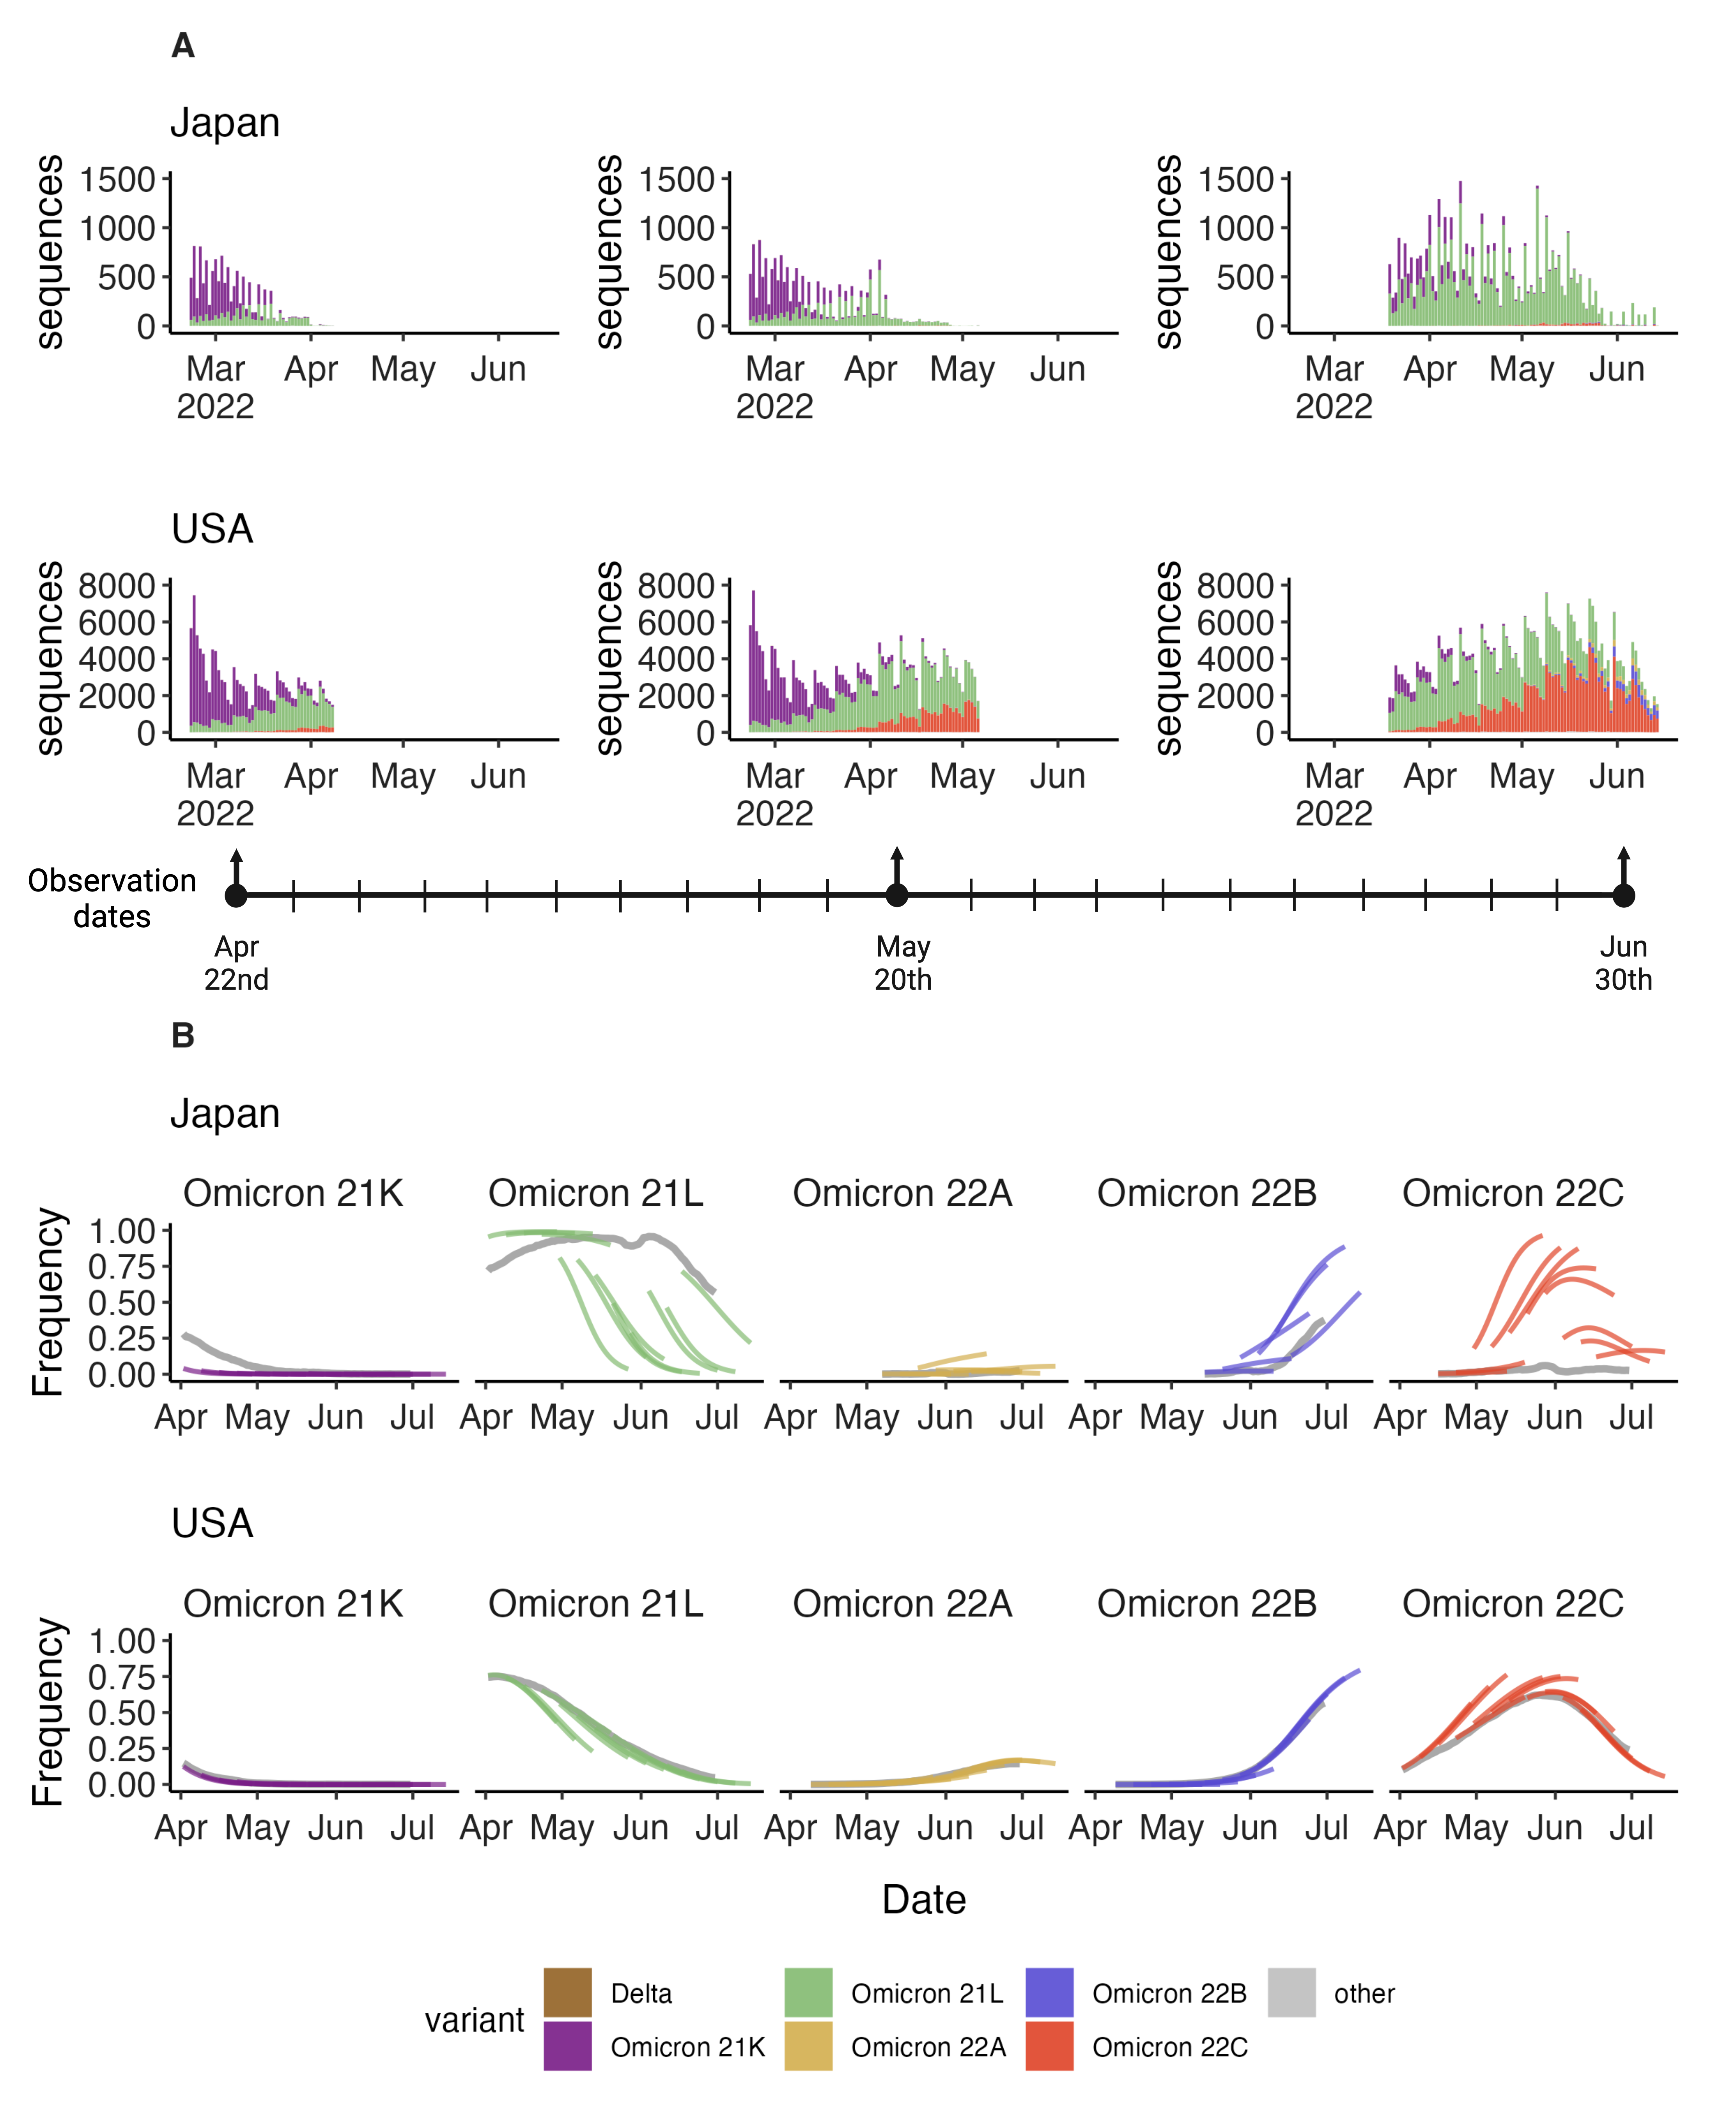
\includegraphics[width=1.0\textwidth]{figures/example_predictions}
	\caption{\textbf{Example data and predictions for Japan and USA.}
	Figure 1 represents a schematic of the dynamic estimation environment, including the progression of dataset estimation, submission delays, and an example estimation of the frequencies of variants using the GARW model. This figure serves as a visual representation of the used methodology
	}
	\label{example_predictions}
\end{figure}


\begin{figure}[h]
	\centering
	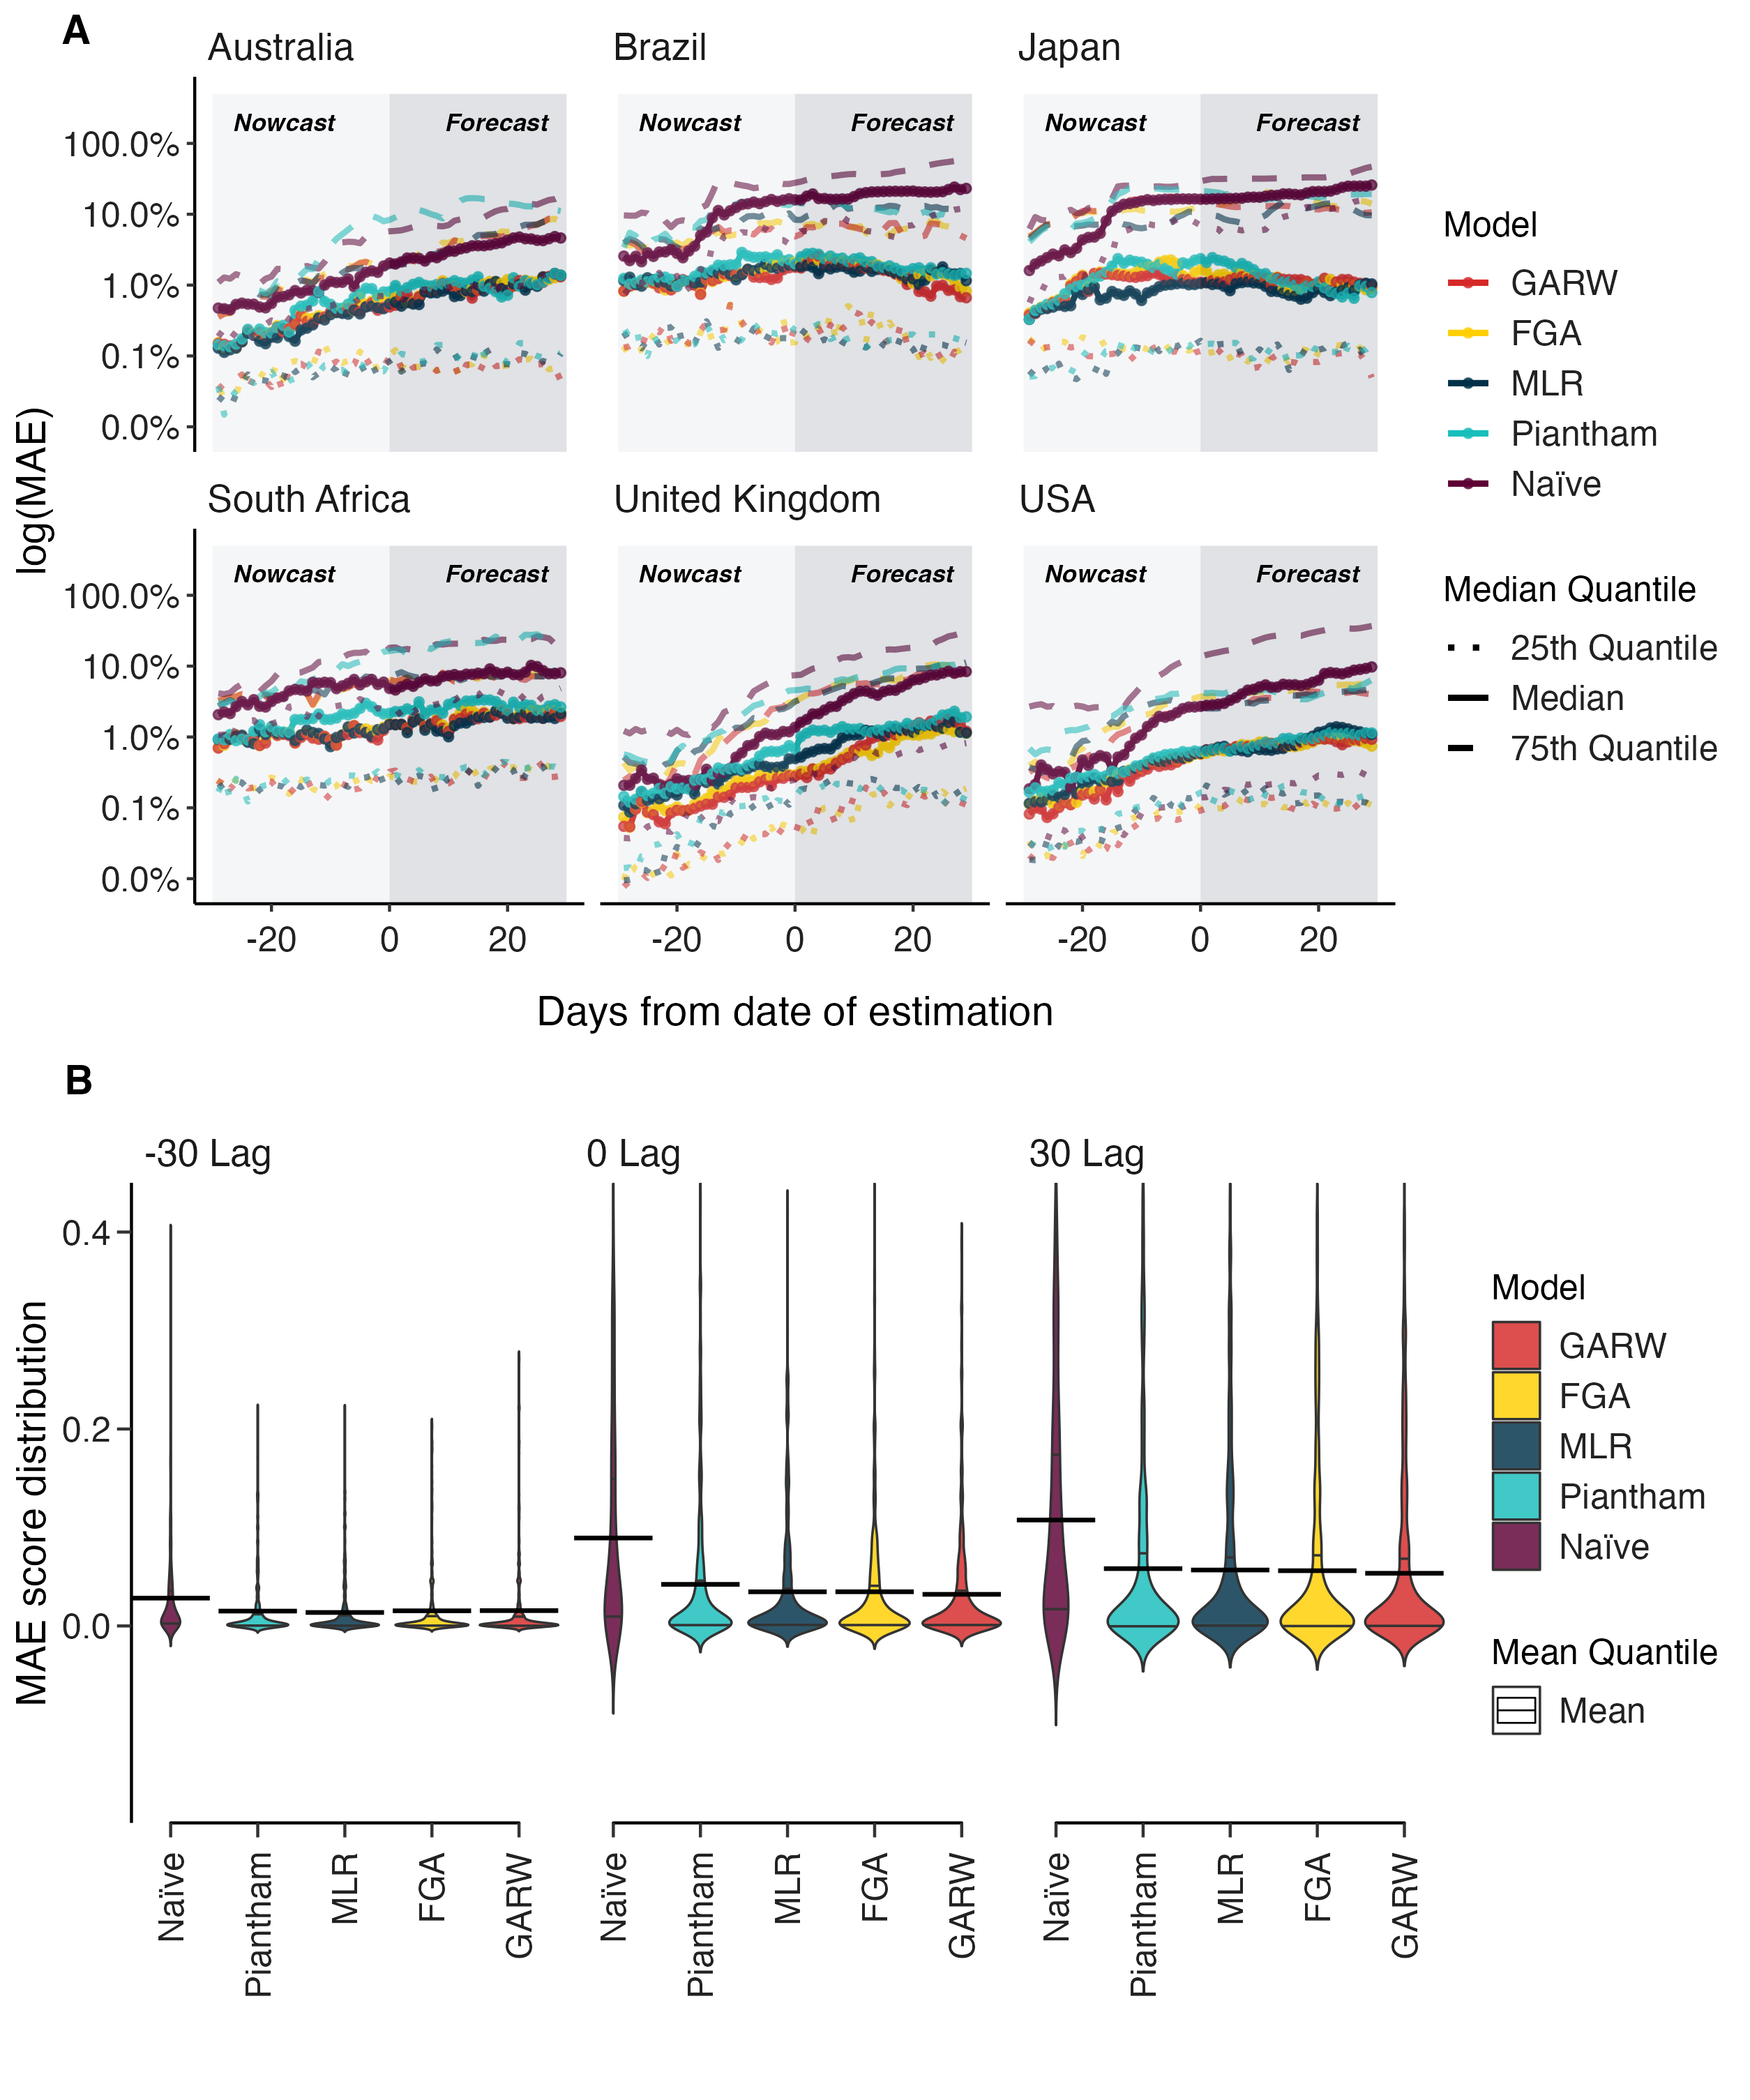
\includegraphics[width=1.0\textwidth]{figures/Figure2.png}
	\caption{\textbf{MAE estimates based on date of estimation.}
	Further legend here.
	}
	\label{Figure 2}
\end{figure}


\begin{figure}[h]
	\centering
	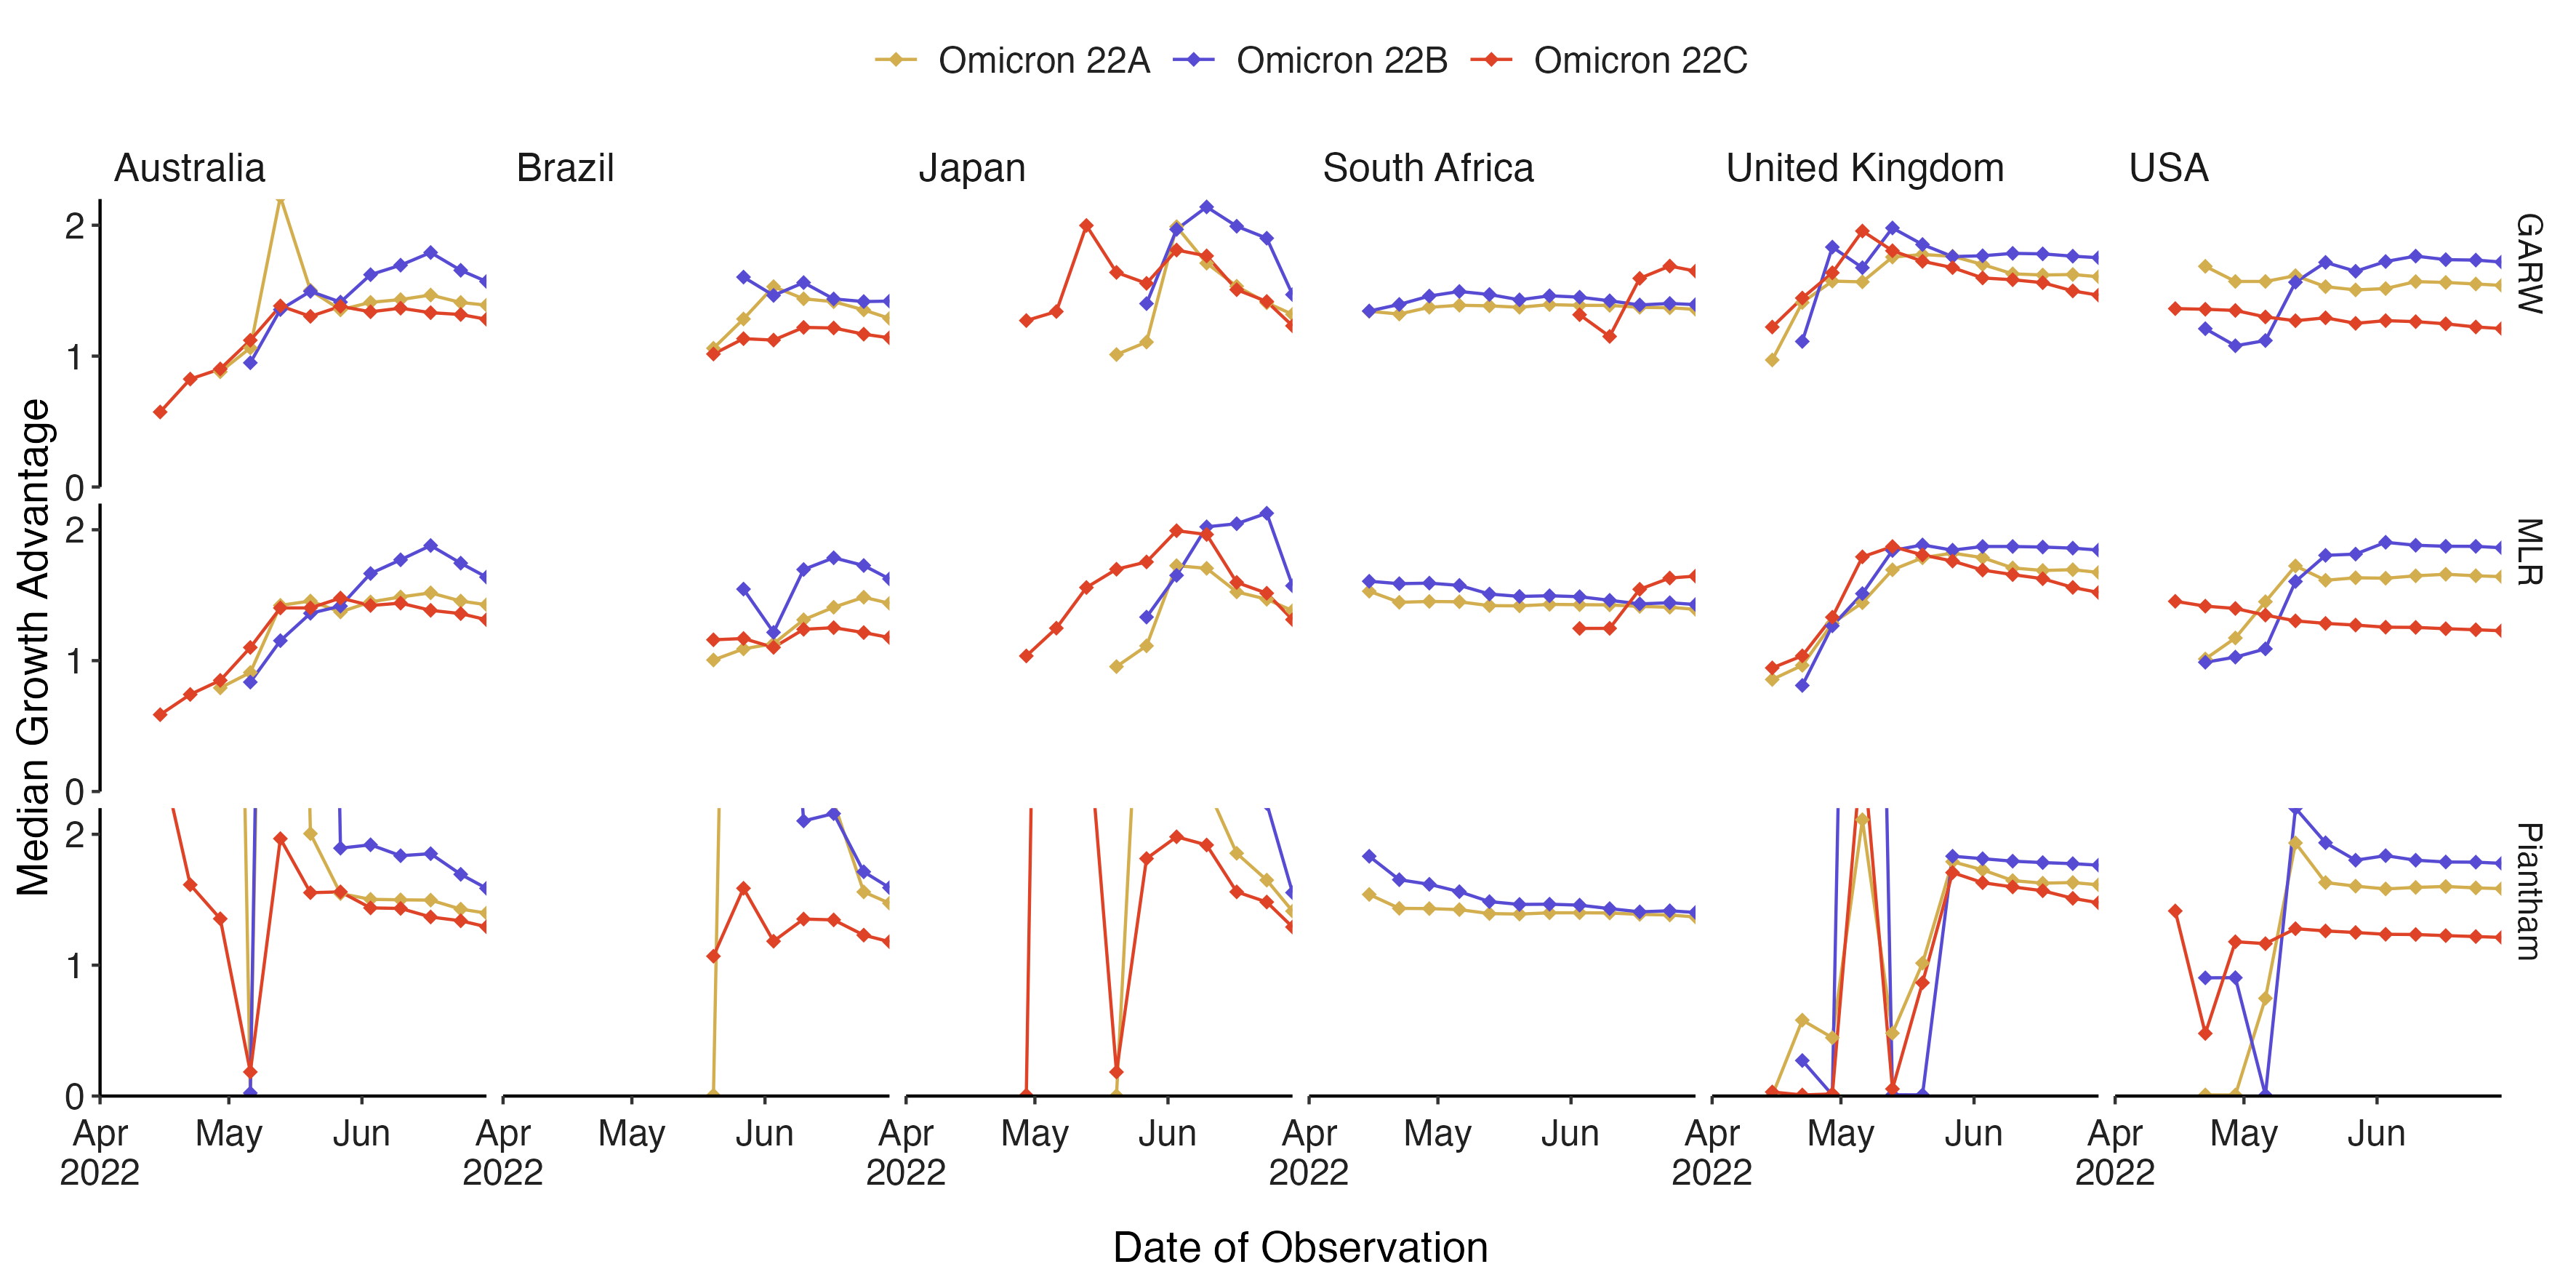
\includegraphics[width=1.0\textwidth]{figures/Figure3.png}
	\caption{\textbf{Growth Advantage of variants over time}
	Further legend here.
	}
	\label{Figure 2}
\end{figure}







%%% DISCUSSION %%%
\section*{Discussion}

Todo

%%% REFERENCES %%%
\bibliographystyle{plos}
\bibliography{ncov-forecasting-fit}

\end{document}
